\documentclass[a4paper]{article}
\usepackage[letterpaper, margin=1in]{geometry} % page format
\usepackage{listings,graphicx,amsmath, amssymb, amsfonts, amsthm, tikz, hyperref, fullpage, setspace, enumerate, mathtools, arydshln, hanging}
\usepackage[english]{babel}

\title{Milestone}
\author{Helen Ngo}
\date{December 20, 2016}

\begin{document}
\lstset{language=Python,basicstyle=\ttfamily\footnotesize}

\maketitle

\begin{doublespace}

\section{Introduction}
The Digit Recognizer is one of the most popular challenges on Kaggle with over 1,300 teams having made submissions. Although engineers and programmers first attempted a handwriting program in 1960s for space industry, ``[t]he qualitative leap in the handwriting recognition market...until [50] year later, due to the massive proliferation of tablets and smartphones? (Shabanova). One of the reasons advancements in handwriting applications may be slow is because many consider writing English slower and more cumbersome than typing. On the other hand, despite markup language LaTeX and its variations, research of post-calculus students found that students felt that typing mathematics can be time consuming and that three-quarters of those students found that LaTeX did not aid them in their understanding of mathematics (Quinlan).

In fact, there is evidence that not only did pen input allow students to record mathematical equations more quickly than typing, it also ``increased transfer to non-computer-based learning tasks such as tests and other assessments? (Anthony). Therefore there remains a need for mathematical handwriting recognition. The traditional applications for handwriting application may have trouble with mathematical symbols since individual subjects require different training, even within mathematics (Anthony). The Digit Recognizer provides the data for this the start of this preliminary research.

Since Kaggle competitors have reached 100\% digit recognition, past research was examined. The numeric system used for the digits were Arabic, but research on Arabic handwriting recognition focused on multidimensional recurrent neural networks was unrealistic to implement. Markov models are used for processing checks, and included an aspect where the data or digits was segmented. Lastly, the Kaggle competition provided a benchmark test with ten thousand records used in random forest training. Having previously used randomForest, this experimentation with this model proved most realistic, but not very hopeful since the benchmark test only correctly classified 93\% of the digits.

\section{Methodology}

Random forest in R was used to examine the digit data. The digits were first tested modified from the code in the benchmark test. Since the real identity of the testing data was unknown, part of the training set was used for testing. 

\lstinputlisting[language=R, firstline=9, lastline=28]{digitrec.R}

By using the the training data for testing, the model also correctly identified approximately 93\% of the digits that it was tested on, confirming that the testing set could be used for training if properly seperated.

Although the training set was limited 42,000 samples for testing, an experiment was conducted to examine if increasing the training could potentially allow for perfect digit recognition. Starting from using a quarter of the training set, 10,500 records, which is about the same amount used in the benchmark test. Five percent increments increases, 2,100 records, were made in the size of the training set each time until 80\% of the total given training set was used or 33,600 records. Each of these training sizes were repeated five times and recorded. Every record that was not used to train with was used to test with, therefore the testing set was always optimized and the model did not become biased to a certain set of digits.

\lstinputlisting[language=R, firstline=30, lastline=41]{digitrec.R}
 
Then only the top 25\% of the most important attributed were used in the model while using the 80\% of the training set in the random forest model; 20\% of the training set was used for testing. It should be noted that only 536 of the 784 attributes has a positive ``MeanDecreaseAccuracy," meaning that only 536 attributes benefited the classification. Therefore the top 25\% or 196 attributes also signified 196 of 536 useful attributes in digit recognition using this data. 

\lstinputlisting[language=R, firstline=64, lastline=69]{digitrec.R}

Finally, it was seen if random forest could differentiate between two numbers, specifically 4 and 9, since those were the most commonly misclassified numbers. This also used the 80/20 split and all the attributes. If successful, a two layer random forest model could be conducted, where the first layer separated the ten digits into groups of commonly misclassified digits, then a second layer focused on more specific attributes to the groups.

\lstinputlisting[language=R, firstline=116 lastline=119]{digitrec.R}

Various experiments were conducted to see if random forest could be the main machine learning tool behind perfect digit classification.

\section{Discussion/Results}

The benchmark test of a training set of 10,000 classified the digits with approximately a 93\% accuracy. By increasing the training set size, the highest accuracy, 0.9577381, achieved using the max number in training, 33,600 records. This training size also achieved the highest average accuracy, 0.9551667, but this was only infinitesimally higher than the average accuracy produced by a training size of 29,400, which was 0.9551464. Accounting for testing size, that's only a few more correctly classified digits despite the thousands more in training. The figure below shows the trend for the expected accuracy given various training sizes; the graph is smoothed to account for outliers.

\begin{center}
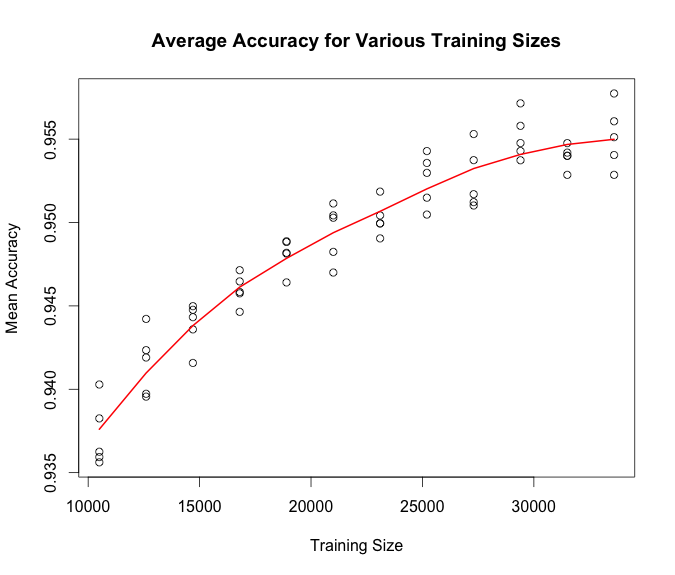
\includegraphics[scale=0.5]{AAVTS.png}
\end{center}

Although 33,600 records gave the highest overall accuracy, it also had a large range of accuracies. Furthermore, the trend of the line begins to level off around 0.955. Therefore perfect accuracy cannot be obtained by simply increasing the training size in random forest, nor can a single known accuracy be obtained for a given training size.

The top 25\% of attributes produced a lower accuracy than the benchmark test, which is to be expected since the most important attribute only increased the accuracy by 0.027437553, and many others by significantly less. Thus every attribute is important and arbitrary at the same time. Using the results from the model that produced the best accuracy, 33,600 records with all attributes, a confusion matrix was produced, showing how the testing set of digits was classified as. Each row represents the distribution of how a single digits was classified, such that [0,1] shows the percentage of zeros that was classified as a one. Note that the main diagonal show the percentage of each digit that was correctly classified with using the model.

\begin{center}
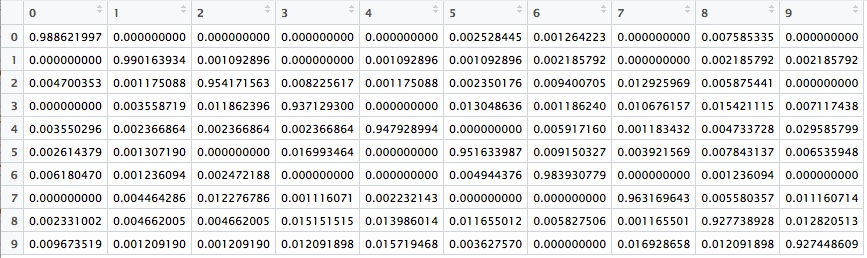
\includegraphics[scale=0.5]{CM.jpeg}
\end{center}

It was expected that 4 and 9 would be commonly misclassified, but it was surprising that 1 and 7 were never misclassified. While 3 and 8 were the most commonly misclassified numbers, 4 and 9 were marginally more misclassified as each other than the former set of digits. In addition, 4 and 9 were less misclassified was other numbers. Overall, the differences between the classification of the two sets of digits were basically insignificant, so 4 and 9 was selected for further examination. Using just two digits, 4 and 9, a random forest model was produced that correctly classified 0.9814593 of the digits. Accounting for the misclassifications with other digits, the overall classification between 4 and 9 seems like it would be only slightly better than a single layer random forest model. Even by reducing the number of different types of digits to two specific digits that the best model had a hard time with, perfect accuracy could not be obtained. If the idea of a two layer random forest was used, the results would still be less can 1.0 classification.

\newpage

\section{Conclusion}
While random forest provides a good benchmark test, it is unlikely that by using random forest alone that a perfect classification of digits could be obtained. Random forest is more like a black box such that specific it's fruitless to isolate specific traits of the data. Using random forest, it seems unlikely to obtain more than 96\% accuracy.

In "A Paradigm for Handwriting-based Intelligent Tutors," Anthony, Yang and Koedinger discuss the importance of a pen input, such as Samsung's S-Pen in mathematical input, but previous Kaggle competitors show that for this specific data set, that's unnecessary. Since I have a concrete understanding of the Markov model, it is used for Arabic handwriting recogontion, and checks have numbers, a modified Markov model would be the next step for further examination. 

\newpage

\section{References/ Bibliography}
\begin{hangparas}{.25in}{1}
Anthony, Lisa, Jie Yang, and Kenneth R. Koedinger. "A Paradigm for Handwriting-based Intelligent Tutors." International Journal of Human-Computer Studies 70.11 (2012): 866-87. Web.

Graves, Alex. "Offline Arabic Handwriting Recognition with Multidimensional Recurrent Neural Networks." Guide to OCR for Arabic Scripts (2012): 297-313. Web.

Konnikova, Maria. "What's Lost as Handwriting Fades." Nytimes.com. The New York Times Company, 2 June 2014. Web. 12 Dec. 2016.

Plotz, Thomas, and Gernot A. Fink. "Markov Models for Offline Handwriting Recognition: A Survey." International Journal on Document Analysis and Recognition (IJDAR) 12.4 (2009): 269-98. Web.

Quinlan, James, and Craig Tennenhouse. "Perceived Utility of Typesetting Homework in Post-Calculus Mathematics Courses." Primus 26.1 (2015): 53-66. Web.
\end{hangparas}
\end{doublespace}
\end{document}
